\chapter{\fancyname{NodeMPST}: Back-End Session Type Web Development}
\label{chap:node}

In this chapter we present \fancyname{NodeMPST},
our session type API generation strategy for 
server-side endpoints. As implied by the name, we assume
that the APIs will be used for implementations running on the
Node.js runtime \cite{Node.js}.

\section{Motivation}
\begin{itemize}
\item session type implementation on the node runtime
\item need to provide consistency under the single-threaded event loop model
\item provide idiomatic event-driven APIs
\item provide static guarantees where possible -- communication mismatch and channel linearity
\end{itemize}

\section{Approach}
\begin{itemize}
\item typescript's type system is gradual, structural and non-linear -- session type api generation examples that provide static guarantees on channel usage build upon target language type system's support for linear resources
\item inspired by purescript approach -- hide the channel resource so they are linear by construction, simply expose callbacks and handlers
\item the runtime executes the EFSM, performs the send and receive actions through the websocket, and invokes the correct handler as required
\item provide overview of the files we generate (and forward reference in the correct subsections) -- EFSM, Runtime, `others' (exclude cancellation)
\end{itemize}

\section{State Encodings}

\begin{itemize}
\item callbacks -- type aliases for each state (handler)
\item need a way for the runtime to distinguish between states
\item attempt at using conditional types, but because they handle conditional union types in a distributed way (give example), cannot be statically typed
\item alternative -- use discriminated union by wrapping in an Implementation class
\item all non-terminal states will `return' the successor implementation -- very difficult to resolve in the type-checker in the runtime (give example of what it may look like) -- solve by giving each state implementation the `advance' function to respect the event-driven nature of everything, so they can call it on completion
\item visualise the interaction between runtime and states as a sequence diagram for message passing
\end{itemize}

\subsection{Send}
\begin{itemize}
\item very short -- go over the structure and give examples
\item show how it extends for polyadic payloads
\end{itemize}

\subsection{Receive}
\begin{itemize}
\item very short -- go over the structure and give examples
\item show how it extends for polyadic payloads
\end{itemize}

\subsection{Terminal}
\begin{itemize}
\item basically nothing here -- can highlight the provided type alias to provide a better developer experience
\end{itemize}

\section{Runtime}
\begin{itemize}
\item public API -- provide seam for websocket server and implementation
\item private API -- carry out the session
\end{itemize}

\subsection{Managing Connections}
\begin{itemize}
\item use set and partial object to keep track of pending connections
\item ws event listeners
\item forward reference that we need to manage cancellations here too
\end{itemize}

\subsection{Executing the EFSM}
\begin{itemize}
\item implementation details delegated to the actual implementation states
\item constructor binds all methods (that will be passed to other components0 to `this' because of how javascript works with respect to the scoping of `this' (give short example -- or ignore, if this is in the background for typescript)
\item advance -- use discriminated union to figure out what to pass to the state (send -- sendMessage, receive -- register)
\end{itemize}

\begin{figure}[!ht]
\centering
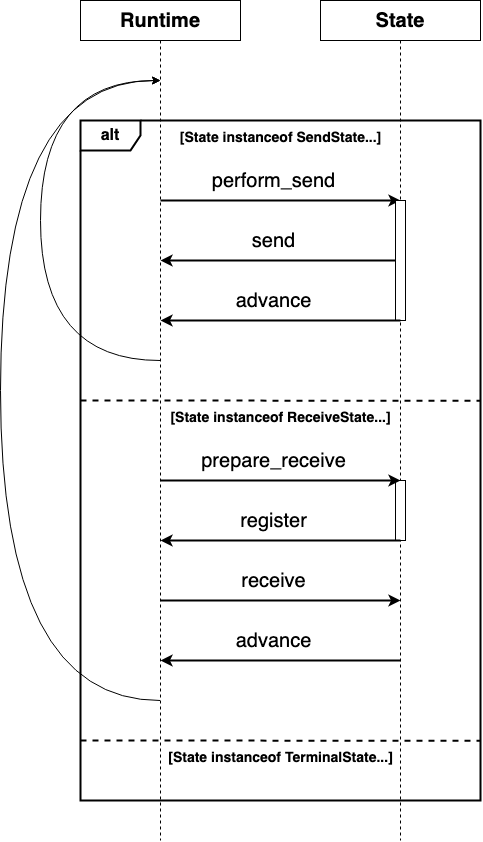
\includegraphics[width=0.5\textwidth]{NodeRuntimeEFSM}
\captionof{figure}{Informal Abstraction of EFSM Execution for
Server Endpoints}
\label{fig:noderuntimeefsm}
\end{figure}

\subsection{Handling Message Sends}
\begin{itemize}
\item very short (just for completeness in the report) -- messages are serialised JS objects (in JSON notation) sent and decoded on the other end, type-correct by construction
\end{itemize}

\subsection{Handling Message Receives}
\begin{itemize}
\item motivate the edge case that message can arrive in the websocket (in succession) before the handler is registered
\item motivate the edge case that message can arrive `out of protocol order' 
\item explain the double queue system and how that provides consistency -- emphasising that this works because of the single-threaded typescript runtime
\end{itemize}

\begin{figure}[!ht]
\centering
\begin{subfigure}[b]{0.8\textwidth}
\centering
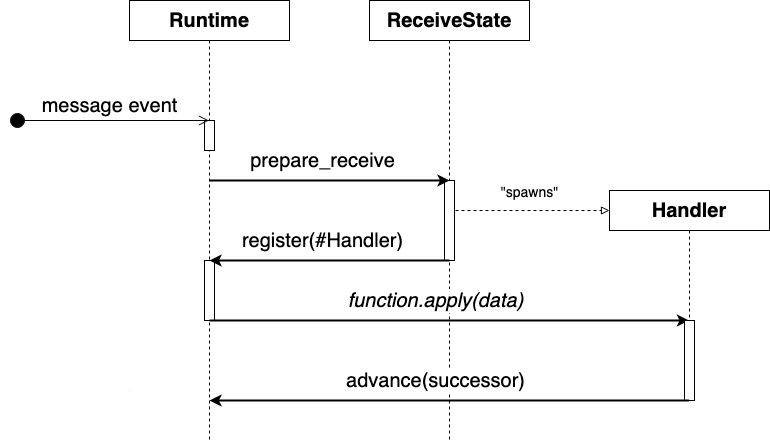
\includegraphics[width=\textwidth]{NodeRuntimeReceive2}
\caption{Message processed before transitioning to receive state}
\label{subfig:nodereceivemsgfirst}
\end{subfigure}
\hfill
\begin{subfigure}[b]{0.8\textwidth}
\centering
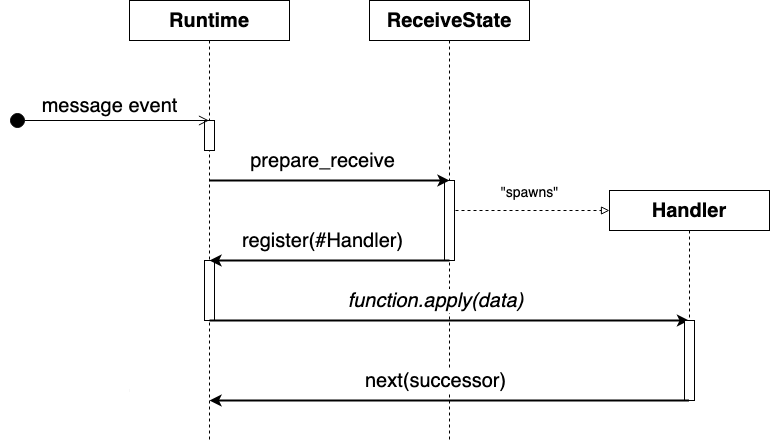
\includegraphics[width=\textwidth]{NodeRuntimeReceive1}
\caption{Message processed after transitioning to receive state}
\label{subfig:nodereceivehandlefirst}
\end{subfigure}
\captionof{figure}{Possible Orderings for Handling Message Event and Preparing
Receive State}
\label{fig:nodereceivecompare}
\end{figure}

\subsection{Handling Termination}
\begin{itemize}
\item design choice that the client is the one that closes the connection because of the centralised role of the server
\item forward reference that this gives opportunity to extend support for general protocols, as in those protocols, the server's terminal state doesn't imply it's terminal for everyone else
\end{itemize}

\section{Alternative Designs and Limitations}

\begin{itemize}
\item exposing channel resources like the java example -- less idiomatic (not-event-driven), need runtime linearity checks like the java example
\item `hardcoded' switch case runtime like the TSOP papers -- doesn't best leverage the type system
\end{itemize}

\section{Summary}
\begin{itemize}
\item static guarantees on channel linearity and communication mismatch (up to the use of `any)
\item handling receives introduce consistency problems, but we deal with it properly here
\end{itemize}